\section{Results}
\label{sec:results}

We first report the size of each bias (\secref{sec:res_main}), then how it changes with scale (\secref{sec:res_scale}) and with the strength of the manipulation (\secref{sec:res_dose}). We close with calibration, the length interaction and the noise floor (\secref{sec:res_calib}).

\subsection{Every Bias Is Much Smaller Than Hypothesised}
\label{sec:res_main}

\begin{figure}[t]
    \centering
    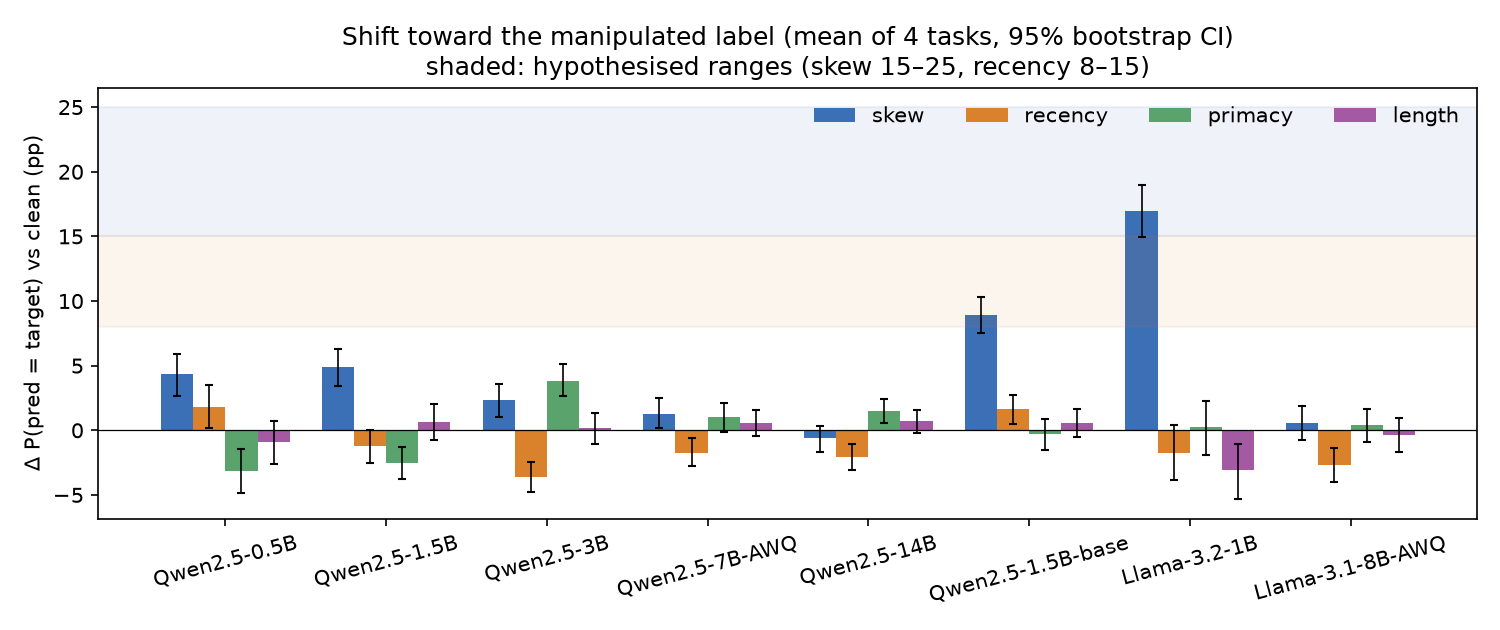
\includegraphics[width=0.95\linewidth]{figures/fig1_target_shift.png}
    \caption{Shift toward the manipulated label $T$ (4-task mean, 95\% bootstrap CIs). The shaded bands mark the hypothesised ranges for skew (15--25 points, blue) and recency (8--15 points, orange). Only \llamaone under frequency skew reaches its band. Recency is negative for every model of 3B and above, and length effects stay within $\pm$3 points.}
    \label{fig:shift}
\end{figure}

\begin{table}[t]
    \centering
    \small
    \begin{tabular}{@{}lcccc@{}}
        \toprule
        \textbf{Model} & \skewc (80/20) & \recency & \primacy & \lengthc \\
        \midrule
        \multicolumn{5}{@{}l}{\emph{\qwen ladder}} \\
        Qwen2.5-0.5B      & \textbf{+4.3}\sig\ {\scriptsize[+2.7, +5.9]} & +1.8\pstar\ {\scriptsize[+0.2, +3.5]} & $-$3.1\sig\ {\scriptsize[$-$4.8, $-$1.5]} & $-$0.9\pstar\ {\scriptsize[$-$2.6, +0.7]} \\
        Qwen2.5-1.5B      & \textbf{+4.9}\sig\ {\scriptsize[+3.4, +6.3]} & $-$1.2\pstar\ {\scriptsize[$-$2.5, $-$0.0]} & $-$2.5\sig\ {\scriptsize[$-$3.8, $-$1.3]} & +0.7\pstar\ {\scriptsize[$-$0.7, +2.0]} \\
        Qwen2.5-3B        & +2.3\sig\ {\scriptsize[+1.1, +3.6]} & $-$3.6\sig\ {\scriptsize[$-$4.8, $-$2.4]} & \textbf{+3.8}\sig\ {\scriptsize[+2.7, +5.1]} & +0.2\pstar\ {\scriptsize[$-$1.0, +1.3]} \\
        Qwen2.5-7B-AWQ    & \textbf{+1.3}\pstar\ {\scriptsize[+0.2, +2.5]} & $-$1.7\sig\ {\scriptsize[$-$2.8, $-$0.6]} & +1.0\pstar\ {\scriptsize[$-$0.1, +2.1]} & +0.6\pstar\ {\scriptsize[$-$0.4, +1.6]} \\
        Qwen2.5-14B       & $-$0.6\pstar\ {\scriptsize[$-$1.7, +0.3]} & $-$2.1\sig\ {\scriptsize[$-$3.1, $-$1.1]} & \textbf{+1.5}\sig\ {\scriptsize[+0.6, +2.4]} & +0.7\pstar\ {\scriptsize[$-$0.2, +1.6]} \\
        \midrule
        \multicolumn{5}{@{}l}{\emph{Base model and second family}} \\
        Qwen2.5-1.5B-base & \textbf{+8.9}\sig\ {\scriptsize[+7.6, +10.3]} & +1.6\pstar\ {\scriptsize[+0.5, +2.7]} & $-$0.3\pstar\ {\scriptsize[$-$1.5, +0.8]} & +0.5\pstar\ {\scriptsize[$-$0.5, +1.6]} \\
        Llama-3.2-1B      & \textbf{+16.9}\sig\ {\scriptsize[+14.9, +19.0]} & $-$1.8\pstar\ {\scriptsize[$-$3.8, +0.4]} & +0.2\pstar\ {\scriptsize[$-$1.9, +2.3]} & $-$3.1\pstar\ {\scriptsize[$-$5.3, $-$1.1]} \\
        Llama-3.1-8B-AWQ  & \textbf{+0.6}\pstar\ {\scriptsize[$-$0.8, +1.8]} & $-$2.7\sig\ {\scriptsize[$-$4.0, $-$1.3]} & +0.4\pstar\ {\scriptsize[$-$0.9, +1.7]} & $-$0.3\pstar\ {\scriptsize[$-$1.7, +1.0]} \\
        \midrule
        \emph{Hypothesised} & +15 to +25 & +8 to +15 & --- & +5 to +10 \\
        \bottomrule
    \end{tabular}
    \caption{Target shift $\shift$ (percentage points) toward the manipulated label, as an equal-weight mean over four tasks, with 95\% cluster-bootstrap CIs. \sig: Holm-adjusted $p<0.05$ over 32 tests. \textbf{Bold}: largest positive shift per model. Only \llamaone under \skewc reaches the hypothesised range. Recency is negative, not positive, for every model of 3B and above.}
    \label{tab:shift}
\end{table}


\Figref{fig:shift} and \tabref{tab:shift} show the main result. {\bf Frequency skew} is the largest bias in every model of 1.5B or smaller: +4.3 and +4.9 points for the small \qwen models, +8.9 for the 1.5B base model and +16.9 for \llamaone. Only \llamaone falls inside the hypothesised 15--25 point range. At 14B and 8B, skew has no detectable effect ($-0.6$ and +0.6).

{\bf Recency} never reaches the predicted 8--15 points. Its largest positive value is +1.8 (Qwen2.5-0.5B), which does not survive Holm correction. From 3B upward the sign flips: two final $T$ demonstrations make the model \emph{less} likely to predict $T$, by $-1.7$ to $-3.6$ points. This holds for all four models of 3B and above, and it is significant after correction in each. {\bf Primacy} roughly mirrors this pattern: it is negative for 0.5B and 1.5B ($-3.1$, $-2.5$) and positive at 3B (+3.8) and 14B (+1.5). {\bf Label--length correlation} has no reliable effect. The largest magnitude is $-3.1$ points (\llamaone), in the direction opposite to the hypothesis, and no length effect survives correction.

\begin{table}[t]
    \centering
    \small
    \begin{tabular}{@{}lccccc@{}}
        \toprule
        & \multicolumn{4}{c}{$\shift$ under \skewc (pp)} & \multirow{2}{*}{\shortstack{Flip rate (\%)\\ \mrpc/mean}} \\
        \cmidrule(lr){2-5}
        \textbf{Model} & \sst & \rte & \agnews & \mrpc & \\
        \midrule
        Qwen2.5-0.5B      & $-$1.2 & $-$3.2 & $-$0.1 & \textbf{+22.0} & 23.0 / 13.1 \\
        Qwen2.5-1.5B      & $-$1.5 & 0.0 & +3.8 & \textbf{+17.2} & 23.5 / \phantom{0}9.4 \\
        Qwen2.5-3B        & +3.0 & $-$0.5 & +1.8 & \textbf{+5.0} & 11.5 / \phantom{0}6.1 \\
        Qwen2.5-7B-AWQ    & +1.0 & $-$1.8 & +0.9 & \textbf{+5.0} & \phantom{0}8.5 / \phantom{0}4.9 \\
        Qwen2.5-14B       & 0.0 & $-$0.5 & \textbf{+0.8} & $-$2.8 & \phantom{0}9.0 / \phantom{0}4.2 \\
        Qwen2.5-1.5B-base & $-$1.5 & +7.8 & +9.8 & \textbf{+19.8} & \phantom{0}6.0 / \phantom{0}6.2 \\
        Llama-3.2-1B      & +3.8 & +22.2 & 0.0 & \textbf{+41.8} & 41.5 / 22.8 \\
        Llama-3.1-8B-AWQ  & $-$0.8 & +2.5 & $-$5.1 & \textbf{+5.8} & 14.5 / \phantom{0}7.8 \\
        \midrule
        Clean acc.\ range (\%) & 89.8--95.5 & 64.2--92.5 & 69.6--85.5 & 54.5--77.0 & \\
        \bottomrule
    \end{tabular}
    \caption{Skew bias by task, and the noise floor. \textbf{Bold}: task with the largest skew shift per model. \sst is essentially immune, while \mrpc, the task with the lowest clean accuracy, carries most of the bias. The last column is the share of predictions that flip when one balanced \clean demonstration set is replaced by another, on \mrpc and averaged over tasks.}
    \label{tab:pertask}
\end{table}


\para{Bias lives in the ambiguous task.} \Tabref{tab:pertask} splits the skew effect by task. \sst, where clean accuracy is 90--96\% for every model, is essentially immune ($|\shift|\le3.8$). \mrpc has the lowest clean accuracy and the highest resampling flip rate, and it carries most of the bias: +17 to +22 points for the small \qwen models, +19.8 for the base model and +41.8 for \llamaone. The 4-task averages in \tabref{tab:shift} therefore understate the risk on hard tasks and overstate it on easy ones.

\para{Where skew hurts.} Because $T$ is rotated, the accuracy that skew adds on items whose gold label is $T$ cancels the accuracy it removes on the others. Overall accuracy therefore changes by at most 2.8 points under any condition (\figref{fig:calib}, right). The split by gold label shows the real cost. For \llamaone, skew lowers accuracy on minority-class items (gold $\neq T$) from 73.3\% to 58.8\% \decrease and raises it on majority-class items from 72.0\% to 86.2\% \increase. The 1.5B base model shows the same pattern (79.8\% $\to$ 70.1\% and 79.2\% $\to$ 88.4\%). Qwen2.5-14B is unaffected (87.2\% $\to$ 87.7\% and 87.1\% $\to$ 86.9\%).

\subsection{Scale Removes Skew and Turns Recency Negative}
\label{sec:res_scale}

\begin{figure}[t]
    \centering
    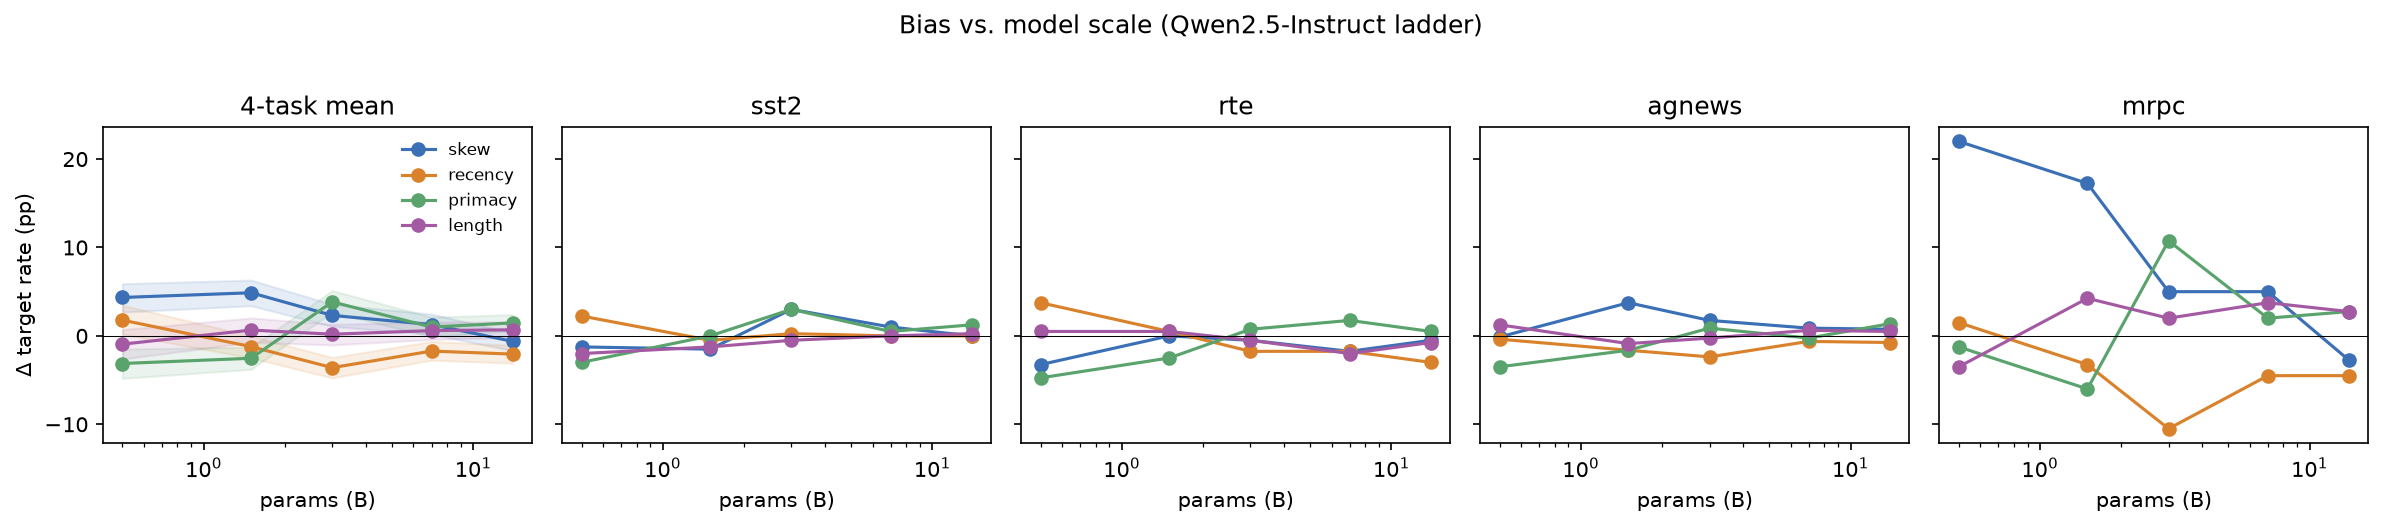
\includegraphics[width=\linewidth]{figures/fig2_scale.png}
    \caption{Target shift against parameter count along the \qwen ladder. Left: 4-task mean with a 95\% CI band. Right: per task. Skew (blue) falls with scale, driven almost entirely by \mrpc. Order effects (recency, orange; primacy, green) are non-monotone and largest at 3B, where \mrpc recency reaches $-10.5$ points.}
    \label{fig:scale}
\end{figure}

\begin{table}[t]
    \centering
    \small
    \begin{tabular}{@{}lccc@{}}
        \toprule
        \textbf{Bias} & \textbf{Slope (pp / decade)} & \textbf{95\% CI} & \textbf{Spearman $\rho$} \\
        \midrule
        \skewc    & $-$3.7 & [$-$4.8, $-$2.4] & $-$0.9 \\
        \recency & $-$2.4 & [$-$3.6, $-$1.2] & $-$0.7 \\
        \primacy & +3.6 & [+2.4, +4.7] & +0.7 \\
        \lengthc & +1.0 & [$-$0.2, +2.2] & +0.7 \\
        \bottomrule
    \end{tabular}
    \caption{OLS slope of $\shift$ on $\log_{10}$(parameters) along the \qwen ladder (five sizes, 0.5B--14B). The CIs reflect item-sampling noise only, not model-to-model variation.}
    \label{tab:slopes}
\end{table}

\Figref{fig:scale} and \tabref{tab:slopes} show how each bias changes along the \qwen ladder. Skew falls by 3.7 points per tenfold increase in parameters ($\rho=-0.9$). The Llama pair agrees: skew drops from +16.9 at 1B to +0.6 at 8B. Recency also falls with scale ($-2.4$ points per decade), but it falls \emph{below zero} rather than rising as H4 predicted. The Llama pair again agrees ($-1.8$ at 1B, n.s.; $-2.7$ at 8B, significant). Primacy rises with scale (+3.6 points per decade). Order effects are not monotone, however: the 3B model shows the largest recency ($-3.6$) and primacy (+3.8) effects of the ladder. The length slope is not distinguishable from zero.

\para{Instruction tuning.} At a fixed size of 1.5B, the base model is about twice as sensitive to skew as its instruction-tuned sibling (+8.9 vs. +4.9 points). It is also the only model besides 0.5B with a positive recency point estimate (+1.6).

\subsection{Large Shifts Require Extreme Manipulations}
\label{sec:res_dose}

\begin{figure}[t]
    \centering
    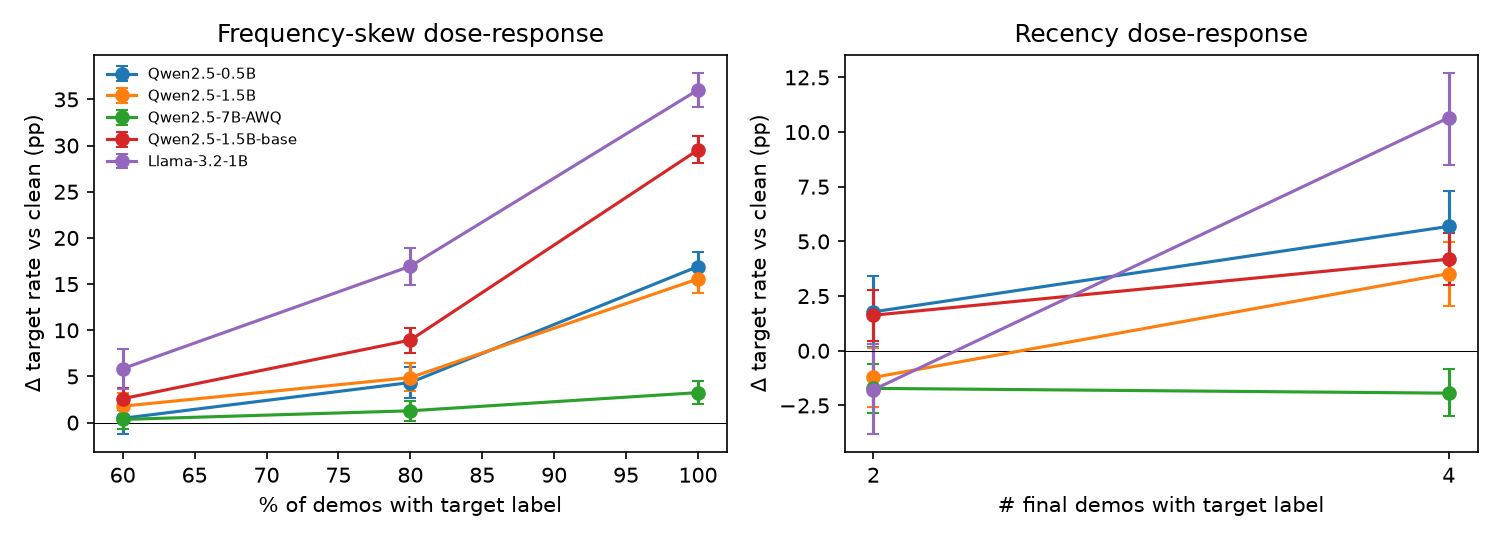
\includegraphics[width=0.85\linewidth]{figures/fig4_dose_response.png}
    \caption{Dose--response on five models. Left: frequency skew at 60\%, 80\% and 100\% target share. Right: recency with the last two or four demonstrations equal to $T$. Skew bias grows sharply once the minority label disappears from the context. Qwen2.5-7B (green) stays nearly flat under both manipulations.}
    \label{fig:dose}
\end{figure}

\begin{table}[t]
    \centering
    \small
    \resizebox{\textwidth}{!}{%
    \begin{tabular}{@{}lccccc@{}}
        \toprule
        & \multicolumn{3}{c}{Frequency skew (share of $T$)} & \multicolumn{2}{c}{Recency (final demos $=T$)} \\
        \cmidrule(lr){2-4} \cmidrule(lr){5-6}
        \textbf{Model} & 60\% & 80\% & 100\% & last 2 & last 4 \\
        \midrule
        Qwen2.5-0.5B      & +0.5 {\scriptsize[$-$1.2, +2.0]} & +4.3 & +16.9 {\scriptsize[+15.4, +18.5]} & +1.8 & +5.7 {\scriptsize[+4.2, +7.3]} \\
        Qwen2.5-1.5B      & +1.8 {\scriptsize[+0.5, +3.2]} & +4.9 & +15.6 {\scriptsize[+14.0, +17.2]} & $-$1.2 & +3.5 {\scriptsize[+2.0, +5.0]} \\
        Qwen2.5-1.5B-base & +2.6 {\scriptsize[+1.5, +3.8]} & +8.9 & +29.5 {\scriptsize[+28.0, +31.0]} & +1.6 & +4.2 {\scriptsize[+3.0, +5.4]} \\
        Llama-3.2-1B      & +5.8 {\scriptsize[+3.7, +7.9]} & +16.9 & \textbf{+36.0} {\scriptsize[+34.1, +38.0]} & $-$1.8 & \textbf{+10.7} {\scriptsize[+8.5, +12.7]} \\
        Qwen2.5-7B-AWQ    & +0.3 {\scriptsize[$-$0.7, +1.4]} & +1.3 & +3.2 {\scriptsize[+2.0, +4.5]} & $-$1.7 & $-$1.9 {\scriptsize[$-$3.0, $-$0.8]} \\
        \bottomrule
    \end{tabular}}
    \caption{Dose--response of target shift $\shift$ (pp, 4-task mean, 95\% CI). The 80\% and last-2 columns repeat \tabref{tab:shift}. Skew bias grows sharply once the minority label disappears from the context. A run of four final $T$ demonstrations produces positive recency in small models but not in Qwen2.5-7B. \textbf{Bold}: largest shift per column group.}
    \label{tab:dose}
\end{table}


\Figref{fig:dose} and \tabref{tab:dose} report the supplementary dose--response set. Skew bias is strongly non-linear. At 60\% target share it is at most +5.8 points; at 80\% it reaches +4 to +17; when all ten demonstrations share one label it jumps to +15.6 to +36.0 points in the small models. The base model again roughly doubles its instruction-tuned sibling (+29.5 vs. +15.6). Most of the skew effect thus appears only when the minority label is (nearly) absent from the context.

Recency behaves differently with longer runs. A run of four final $T$ demonstrations gives a positive recency effect in all small models (+3.5 to +10.7), including 1.5B and \llamaone, where a run of two had a negative point estimate. {\bf Qwen2.5-7B is almost immune to both extreme doses.} All-$T$ demonstrations move it by only +3.2 points, and four final $T$ demonstrations still produce anti-recency ($-1.9$). Scale therefore removes not only the moderate biases but most of the dose--response.

\subsection{Calibration, Length Interaction and Noise Floor}
\label{sec:res_calib}

\begin{figure}[t]
    \centering
    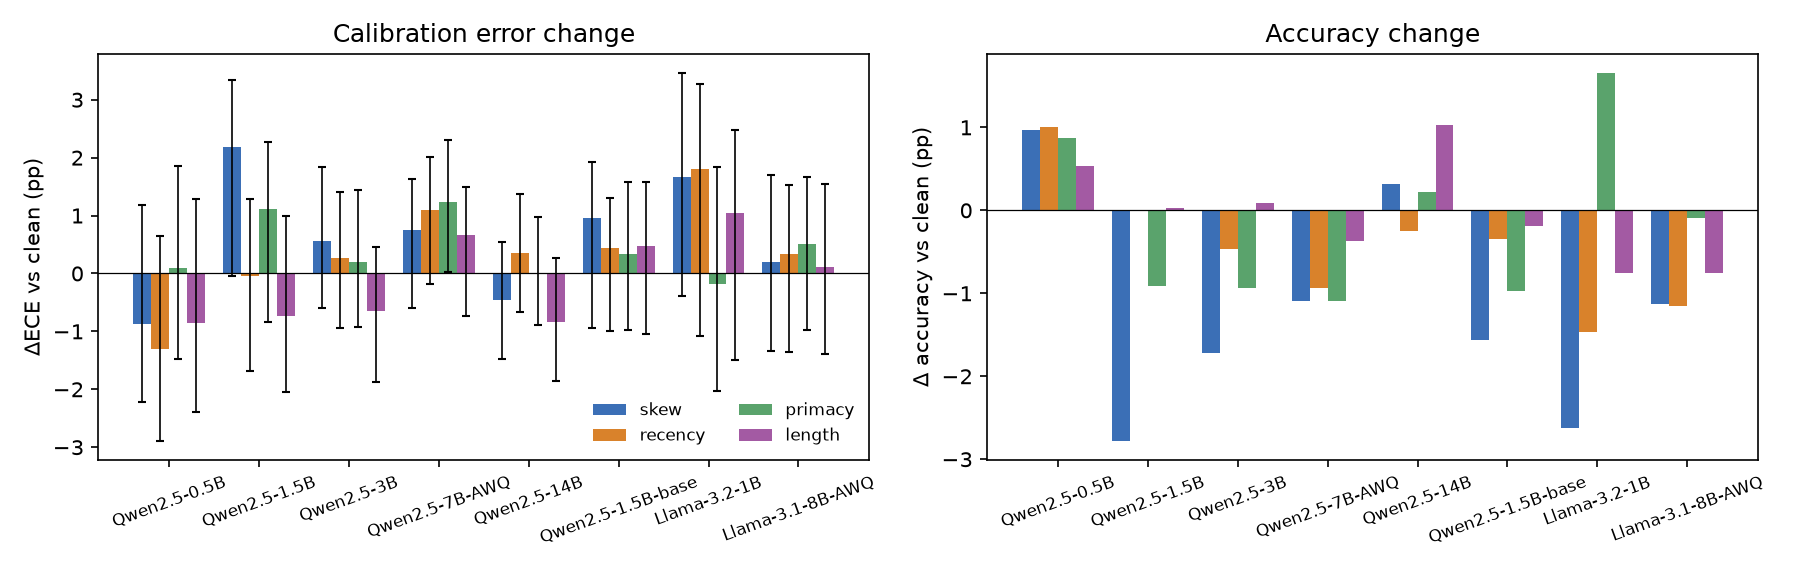
\includegraphics[width=0.95\linewidth]{figures/fig3_calibration_accuracy.png}
    \caption{Left: change in ECE against \clean, with paired bootstrap 95\% CIs. Right: change in overall accuracy. Only one of 32 $\Delta$ECE intervals excludes zero, and overall accuracy moves by less than 3 points, because target rotation makes the gains and losses cancel.}
    \label{fig:calib}
\end{figure}

\begin{table}[t]
    \centering
    \small
    \begin{tabular}{@{}lccccccc@{}}
        \toprule
        & \multicolumn{5}{c}{ECE} & \multicolumn{2}{c}{Norm.\ entropy} \\
        \cmidrule(lr){2-6} \cmidrule(lr){7-8}
        \textbf{Model} & \clean & \skewc & \recency & \primacy & \lengthc & \clean & \skewc \\
        \midrule
        Qwen2.5-0.5B      & .071 & .062 & .058 & .072 & .062 & .575 & .569 \\
        Qwen2.5-1.5B      & .049 & .070 & .048 & .060 & .041 & .427 & .433 \\
        Qwen2.5-3B        & .121 & .127 & .124 & .123 & .114 & .170 & .185 \\
        Qwen2.5-7B-AWQ    & .111 & .118 & .121 & .123$^{\dagger}$ & .117 & .105 & .118 \\
        Qwen2.5-14B       & .097 & .092 & .101 & .097 & .089 & .099 & .102 \\
        Qwen2.5-1.5B-base & .058 & .067 & .062 & .061 & .063 & .540 & .537 \\
        Llama-3.2-1B      & .035 & .051 & .053 & .033 & .045 & .651 & .645 \\
        Llama-3.1-8B-AWQ  & .053 & .055 & .056 & .058 & .055 & .337 & .357 \\
        \bottomrule
    \end{tabular}
    \caption{Expected calibration error (equal-task mean) and normalised predictive entropy. $\Delta$ECE against \clean lies between $-1.3$ and $+2.2$ points. 9 of 32 differences are negative, and only one paired bootstrap CI excludes zero ($^{\dagger}$: +1.2 [+0.02, +2.3], before correcting for 32 comparisons). Differences between models (larger Qwen models are overconfident even on \clean prompts) are much larger than differences between conditions.}
    \label{tab:calibration}
\end{table}


\para{Calibration does not degrade.} \Tabref{tab:calibration} and \figref{fig:calib} show that $\Delta$ECE ranges from $-1.3$ to +2.2 points. Nine of the 32 point estimates are negative. Only one CI excludes zero (Qwen2.5-7B, \primacy: +1.2 [+0.02, +2.3]), and only before correcting for multiple comparisons. The largest point estimate, Qwen2.5-1.5B under skew (+2.2 [$-0.05$, +3.3]), does not. Normalised entropy barely moves (\eg 0.099 vs. 0.102 for 14B under skew). The larger difference is between models: \qwen models of 3B and above are overconfident even on \clean prompts (ECE 0.10--0.12, against 0.05--0.07 for 0.5B and 1.5B). This is a property of the models, not of the manipulations.

\para{No length rule.} If the \lengthc condition taught a ``long input $\to T$'' rule, the shift would be larger for long test inputs (above the task median) than for short ones. The long-minus-short difference ranges from $-0.6$ to +1.9 points, and every 95\% CI contains zero. The models did not learn a length-to-label association, even though $T$ demonstrations were 15--29 words longer on average.

\para{The noise floor dominates in larger models.} Re-drawing a balanced \clean demonstration set flips 4.2\% (Qwen2.5-14B) to 22.8\% (\llamaone) of predictions, and up to 41.5\% on \mrpc for \llamaone (\tabref{tab:pertask}). For every model of 3B and above, this ordinary resampling instability (4.2--7.8\%) is larger than any systematic bias in \tabref{tab:shift} (at most 3.8 points).

\begin{table}[t]
    \centering
    \small
    \begin{tabular}{@{}lp{3.3cm}p{5.4cm}l@{}}
        \toprule
        & \textbf{Prediction} & \textbf{Result} & \textbf{Verdict} \\
        \midrule
        H1  & skew largest, 15--25 pp & largest in all models $\le$1.5B (4.3--16.9 pp); only \llamaone in range; $\approx$0 at 8--14B & partly supported \\
        H2  & recency second, 8--15 pp & $\le$+1.8 pp; significantly negative ($-1.7$ to $-3.6$) at $\ge$3B & refuted \\
        H3  & length 5--10 pp, scale-resistant & $|\shift|\le3.1$, none significant; no length rule & refuted \\
        H4a & scale corrects skew & $-3.7$ pp/decade; Llama 16.9 $\to$ 0.6 & supported \\
        H4b & scale amplifies recency & recency turns negative with scale & refuted \\
        H5  & ECE rises under every bias & 1/32 CIs above 0 (uncorrected); 9/32 negative & refuted \\
        \bottomrule
    \end{tabular}
    \caption{Verdicts on the five hypotheses.}
    \label{tab:verdicts}
\end{table}

\para{Summary.} \Tabref{tab:verdicts} collects the verdicts. Only the claim that scale corrects frequency skew is fully supported. The claim that skew is the largest bias holds for small models, but its magnitude is far below the prediction for instruction-tuned models.
